\documentclass[tikz,border=15pt]{standalone}
\usepackage{tikz}
\usetikzlibrary{shapes.geometric, arrows.meta, positioning, calc, backgrounds, fit}

\begin{document}
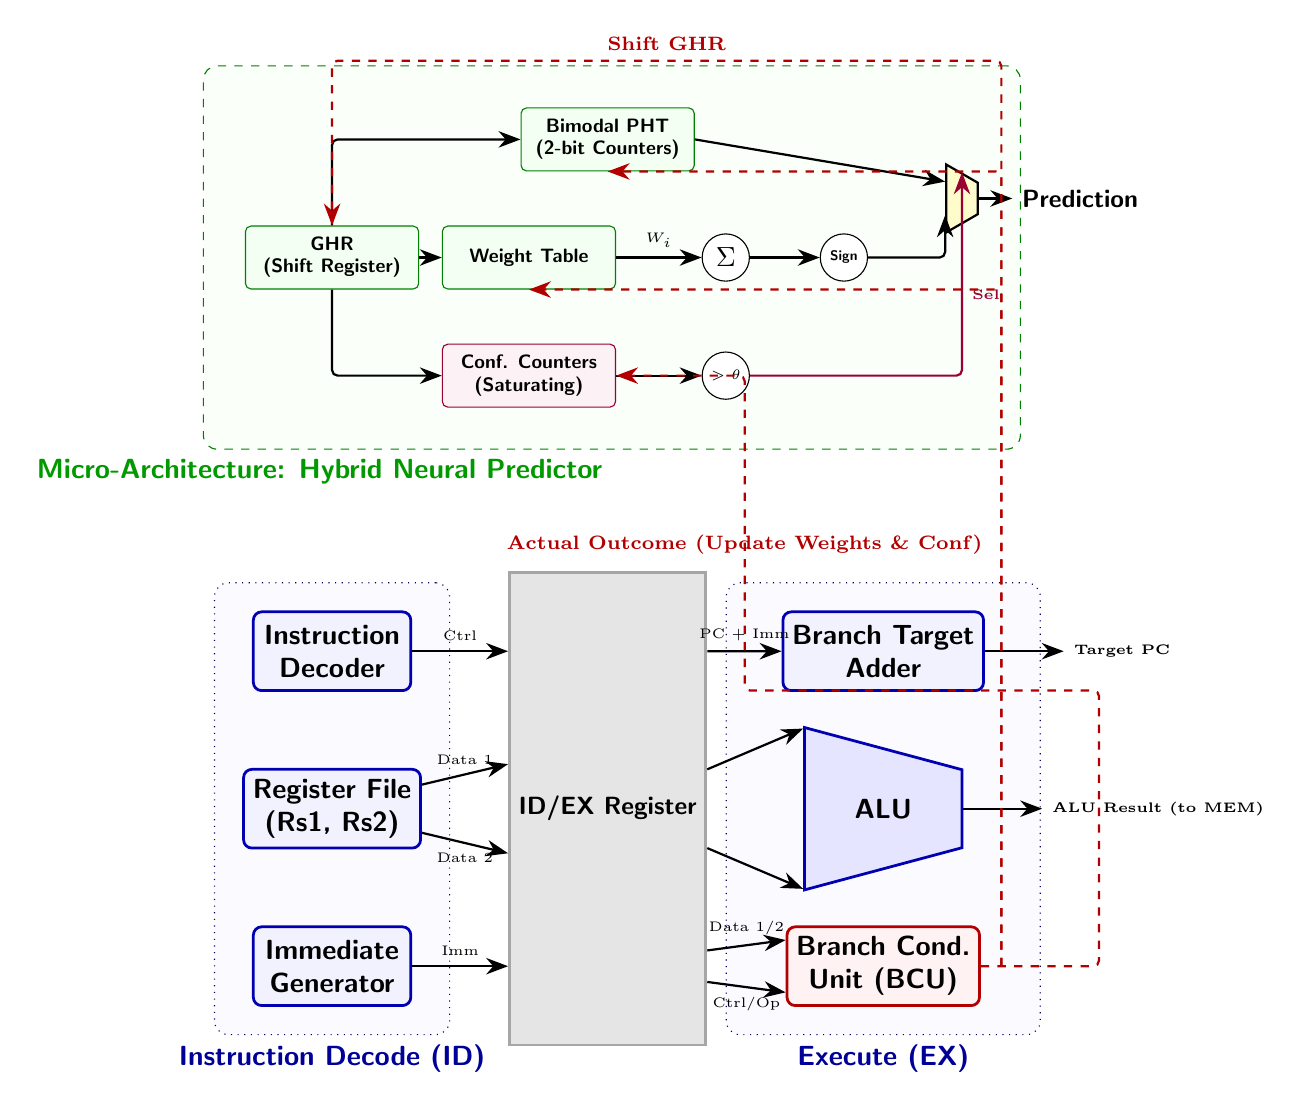
\begin{tikzpicture}[
  font=\sffamily\small,
  every node/.style={align=center},
  %% ─── 樣式定義 ────────────────────────────────────────────────
  block/.style={
    draw=blue!70!black, fill=blue!5, rounded corners=3pt,
    minimum width=2cm, minimum height=1cm, line width=1pt, font=\sffamily\bfseries
  },
  alu/.style={
    draw=blue!70!black, fill=blue!10,
    trapezium, trapezium angle=75, shape border rotate=270,
    minimum width=1.5cm, minimum height=2cm, line width=1pt, font=\sffamily\bfseries
  },
  pipereg/.style={
    draw=gray!70, fill=gray!20,
    minimum width=0.6cm, minimum height=6cm, line width=1pt, font=\sffamily\small\bfseries
  },
  predblock/.style={
    draw=green!50!black, fill=green!5, rounded corners=2pt,
    minimum width=2.2cm, minimum height=0.8cm, font=\sffamily\scriptsize\bfseries
  },
  mathnode/.style={
    circle, draw=black, fill=white, inner sep=1pt, minimum size=0.6cm, font=\sffamily\bfseries
  },
  mux/.style={
    draw=black, fill=yellow!20,
    trapezium, trapezium angle=60, shape border rotate=270,
    minimum width=0.8cm, minimum height=0.4cm, line width=0.8pt
  },
  darrow/.style={-{Stealth[scale=1.2]}, thick, rounded corners=2pt},
  uarrow/.style={dashed, -{Stealth[scale=1.2]}, thick, red!70!black, rounded corners=2pt}
]

  %% ─── 1. ID Stage 展開 (X=0) ──────────────────────────────────
  \node[block] (Decoder) at (0, 2) {Instruction\\Decoder};
  \node[block] (RegFile) at (0, 0) {Register File\\(Rs1, Rs2)};
  \node[block] (ImmGen) at (0, -2) {Immediate\\Generator};

  %% ─── 2. ID/EX Pipeline Register (X=3.5) ──────────────────────
  \node[pipereg] (IDEX) at (3.5, 0) {ID/EX Register};

  % ID 到 IDEX 的連線
  \draw[darrow] (Decoder.east) -- (Decoder -| IDEX.west) node[midway, above, font=\tiny] {Ctrl};
  \draw[darrow] (RegFile.15) -- ([yshift=0.26cm]IDEX.west |- RegFile.15) node[midway, above, font=\tiny] {Data 1};
  \draw[darrow] (RegFile.345) -- ([yshift=-0.26cm]IDEX.west |- RegFile.345) node[midway, below, font=\tiny] {Data 2};
  \draw[darrow] (ImmGen.east) -- (ImmGen -| IDEX.west) node[midway, above, font=\tiny] {Imm};

  %% ─── 3. EX Stage 展開 (X=7) ──────────────────────────────────
  \node[block] (BrAdder) at (7, 2) {Branch Target\\Adder};
  \node[alu] (ALU) at (7, 0) {ALU};
  \node[block, draw=red!70!black, fill=red!5] (BCU) at (7, -2) {Branch Cond.\\Unit (BCU)};

  % IDEX 到 EX 的連線
  \draw[darrow] ([yshift=2cm]IDEX.east) -- (BrAdder.west) node[midway, above, font=\tiny] {PC + Imm};
  
  \draw[darrow] ([yshift=0.5cm]IDEX.east) -- (ALU.north west);
  \draw[darrow] ([yshift=-0.5cm]IDEX.east) -- (ALU.south west);
  
  \draw[darrow] ([yshift=-1.8cm]IDEX.east) -- (BCU.165) node[midway, above, font=\tiny] {Data 1/2};
  \draw[darrow] ([yshift=-2.2cm]IDEX.east) -- (BCU.195) node[midway, below, font=\tiny] {Ctrl/Op};

  % EX 輸出
  \draw[darrow] (ALU.east) -- ++(1,0) node[right, font=\tiny\bfseries] {ALU Result (to MEM)};
  \draw[darrow] (BrAdder.east) -- ++(1,0) node[right, font=\tiny\bfseries] {Target PC};

  %% ─── 4. Branch Predictor 微架構展開 (Y=6.5 至 Y=9, 橫跨 X=1 到 X=8) ─────
  \node[predblock] (GHR) at (0, 7) {GHR\\(Shift Register)};
  
  % Bimodal Path
  \node[predblock] (Bimodal) at (3.5, 8.5) {Bimodal PHT\\(2-bit Counters)};
  
  % Perceptron Path (展開)
  \node[predblock] (PTable) at (2.5, 7) {Weight Table};
  \node[mathnode] (Dot) at (5, 7) {$\Sigma$};
  \node[mathnode, font=\sffamily\tiny\bfseries] (Sign) at (6.5, 7) {Sign};
  
  % Confidence Path (展開)
  \node[predblock, draw=purple!80!black, fill=purple!5] (ConfTable) at (2.5, 5.5) {Conf. Counters\\(Saturating)};
  \node[mathnode, font=\sffamily\tiny\bfseries] (Thresh) at (5, 5.5) {$>\theta$};

  % MUX & Output
  \node[mux] (PredMUX) at (8, 7.75) {};
  \node[font=\sffamily\small\bfseries] (FinalPred) at (9.5, 7.75) {Prediction};

  % Predictor 內部連線
  \draw[darrow] (GHR.north) |- (Bimodal.west);
  \draw[darrow] (GHR.east) -- (PTable.west);
  \draw[darrow] (GHR.south) |- (ConfTable.west);

  \draw[darrow] (PTable.east) -- (Dot.west) node[midway, above, font=\tiny] {$W_i$};
  \draw[darrow] (Dot.east) -- (Sign.west);
  
  \draw[darrow] (ConfTable.east) -- (Thresh.west);

  \draw[darrow] (Bimodal.east) -- (PredMUX.north west);
  \draw[darrow] (Sign.east) -| (PredMUX.south west);

  % 信心選擇訊號
  \draw[darrow, purple!80!black, thick] (Thresh.east) -| (PredMUX.north) node[pos=0.7, right, font=\tiny\bfseries] {Sel};
  \draw[darrow] (PredMUX.east) -- (FinalPred.west);

  %% ─── 5. EX 階段回饋更新 (Update Path) ────────────────────────
  % 從 BCU 擷取真實分支結果，向上穿越回傳給 Predictor 更新權重
  \draw[uarrow] (BCU.east) -- ++(1.5,0) -- ++(0, 3.5) -- ++(-4.5, 0) |- (ConfTable.east) node[pos=0.2, above, font=\scriptsize\bfseries] {Actual Outcome (Update Weights \& Conf)};
  \draw[uarrow] (8.5, -2) -- (8.5, 5.5) |- (PTable.south);
  \draw[uarrow] (8.5, -2) -- (8.5, 5.5) |- (Bimodal.south);
  \draw[uarrow] (8.5, -2) -- (8.5, 5.5) -- (8.5, 9.5) -| (GHR.north) node[pos=0.25, above, font=\scriptsize\bfseries] {Shift GHR};

  %% ─── 6. 封裝背景框 ──────────────────────────────────────────
  \begin{scope}[on background layer]
    % ID Box
    \node[draw=blue!40!black, dotted, fill=blue!2, rounded corners=5pt, inner sep=10pt, fit=(Decoder) (RegFile) (ImmGen), label={[font=\sffamily\bfseries, blue!60!black]below:Instruction Decode (ID)}] {};
    % EX Box
    \node[draw=blue!40!black, dotted, fill=blue!2, rounded corners=5pt, inner xsep=20pt, inner ysep=10pt, fit=(BrAdder) (ALU) (BCU), label={[font=\sffamily\bfseries, blue!60!black]below:Execute (EX)}] {};
    % Predictor Box
    \node[draw=green!50!black, dashed, fill=green!2, rounded corners=5pt, inner xsep=15pt, inner ysep=15pt, fit=(GHR) (Bimodal) (PTable) (Dot) (Sign) (ConfTable) (Thresh) (PredMUX), label={[font=\sffamily\bfseries, green!60!black, anchor=north east]south:Micro-Architecture: Hybrid Neural Predictor}] {};
  \end{scope}

\end{tikzpicture}
\end{document}